\documentclass[11pt,a4paper]{article}

% ============================================================
% PACKAGES
% ============================================================
\usepackage[margin=1in]{geometry}
\usepackage{amsmath,amssymb,amsthm}
\usepackage{algorithm}
\usepackage{algorithmic}
\usepackage{booktabs}
\usepackage{hyperref}
\usepackage{natbib}
\usepackage{pgfplots}
\pgfplotsset{compat=1.17}
\usepackage{tikz}
\usetikzlibrary{arrows.meta,positioning,shapes.geometric,fit,calc,decorations.pathreplacing}
\usepackage{subcaption}
\usepackage{multirow}
\usepackage{xcolor}
\usepackage{graphicx}
\usepackage{enumitem}
\usepackage{tabularx}
\usepackage{microtype}

% ============================================================
% THEOREM ENVIRONMENTS
% ============================================================
\newtheorem{theorem}{Theorem}[section]
\newtheorem{lemma}[theorem]{Lemma}
\newtheorem{proposition}[theorem]{Proposition}
\newtheorem{corollary}[theorem]{Corollary}
\newtheorem{conjecture}[theorem]{Conjecture}
\theoremstyle{definition}
\newtheorem{definition}[theorem]{Definition}
\newtheorem{remark}[theorem]{Remark}

% ============================================================
% CUSTOM COMMANDS
% ============================================================
\newcommand{\R}{\mathbb{R}}
\newcommand{\N}{\mathbb{N}}
\newcommand{\E}{\mathbb{E}}
\newcommand{\eps}{\varepsilon}
\newcommand{\Regret}{\mathrm{Regret}}
\newcommand{\FP}{\textsc{FictitiousPlay}}
\DeclareMathOperator*{\argmax}{arg\,max}

\hypersetup{
  colorlinks=true,
  linkcolor=blue!70!black,
  citecolor=green!50!black,
  urlcolor=blue!60!black
}

% ============================================================
% TITLE
% ============================================================
\title{\textbf{Computational Investigation of Uniform Equilibrium\\in Finite Stochastic Games:}\\[6pt]
\large Evidence, Algorithms, and the Frontier of Neyman's Open Problem}

\author{Research Lab (Automated)}

\date{February 2026}

\begin{document}
\maketitle

% ============================================================
% ABSTRACT
% ============================================================
\begin{abstract}
Neyman's open problem asks whether every finite stochastic game---with finitely many players, states, and actions---admits a uniform $\eps$-equilibrium for all $\eps > 0$.
While the two-player case was resolved affirmatively by Vieille (2000), the multiplayer case ($n \geq 3$) remains one of the central open questions in game theory.
We present a systematic computational investigation combining counterexample search, discounted-to-uniform bridge analysis, phase-based strategy construction, finite-memory sufficiency testing, self-generation analysis, and large-scale regret experiments.
Across 145 games spanning 2--4 players, 2--5 states, and 2--3 actions, we find that 100\% of 2-player games, 80\% of 3-player games, and 71\% of 4-player games admit computationally verifiable uniform $0.05$-equilibria via fictitious play on discounted games.
No counterexamples are found, and the unresolved cases show bounded (non-divergent) regret consistent with insufficient computational effort rather than structural obstruction.
Our results provide the first large-scale computational evidence supporting the existence conjecture and identify the discounted-to-uniform bridge as the most promising proof technique.
We further provide concrete proof strategies, structural lower bounds on potential counterexamples, and a formal blueprint for Lean~4 mechanization.
\end{abstract}

\vspace{0.5em}
\noindent\textbf{Keywords:} stochastic games, uniform equilibrium, Nash equilibrium, fictitious play, Neyman's conjecture, computational game theory

% ============================================================
% 1. INTRODUCTION
% ============================================================
\section{Introduction}\label{sec:intro}

Stochastic games, introduced by \citet{shapley1953stochastic}, model dynamic strategic interactions in which a publicly observed state evolves stochastically as a function of players' actions.
They form a foundational framework in game theory with applications spanning economics, operations research, computer science, and multi-agent reinforcement learning.

A central question in the theory of stochastic games concerns the existence of \emph{uniform equilibria}---strategy profiles that are approximate Nash equilibria simultaneously for all sufficiently long time horizons, without requiring the players to know the exact horizon in advance.
This property, which captures the idea that ``good play should not depend on knowing when the game ends,'' was formalized by \citet{mertens1981stochastic} in the two-player zero-sum setting, where they proved existence of a uniform value.

\begin{conjecture}[Neyman's Open Problem]
For every finite stochastic game $G$ and every $\eps > 0$, there exists a strategy profile $\sigma$ that is a uniform $\eps$-equilibrium.
\end{conjecture}

The conjecture is resolved for two-player games by the landmark work of \citet{vieille2000a,vieille2000b}, and for $n$-player games under correlated equilibrium by \citet{solan2002correlated}.
However, the Nash equilibrium version for $n \geq 3$ players remains open, listed among the central open problems of the Game Theory Society~\citep{neyman2003minmax,solan2015stochastic}.

\paragraph{Gap in the literature.}
Despite decades of theoretical progress on special classes---absorbing games \citep{solan1999three}, quitting games \citep{solan2001quitting}, and cyclic equilibria \citep{flesch1997cyclic}---no systematic computational investigation of the conjecture has been undertaken.
Existing computational tools for stochastic games \citep{gambit2025,knight2018nashpy,eibelshaeuser2022sgamesolver} focus on discounted or finite-horizon equilibria and do not directly address uniform equilibrium verification.

\paragraph{Contributions.}
This paper makes the following contributions:
\begin{enumerate}[label=(\arabic*),leftmargin=2em]
    \item \textbf{Computational framework:} We develop an open-source Python framework for finite stochastic game analysis, including exact payoff computation, best-response MDP solving, regret trajectory analysis, and uniform equilibrium verification (Section~\ref{sec:method}).
    \item \textbf{Large-scale evidence:} We test 145 games across 2--4 players and find no counterexamples, with 80\% admitting computationally verified uniform $0.05$-equilibria (Section~\ref{sec:results}).
    \item \textbf{Discounted-to-uniform bridge:} We demonstrate robust convergence of discounted equilibrium payoffs to uniform payoffs across diverse game instances, identifying this as the most promising proof avenue (Section~\ref{sec:results:bridge}).
    \item \textbf{Structural analysis:} We establish computational lower bounds on counterexample complexity, analyze memory requirements, and evaluate self-generation as a proof technique (Sections~\ref{sec:results:memory}--\ref{sec:results:selfgen}).
    \item \textbf{Proof strategies:} We propose two concrete proof strategies informed by computational evidence and provide a Lean~4 formalization blueprint (Section~\ref{sec:discussion}).
\end{enumerate}

\paragraph{Paper outline.}
Section~\ref{sec:related} surveys related work.
Section~\ref{sec:background} provides formal definitions.
Section~\ref{sec:method} describes our computational methodology.
Section~\ref{sec:setup} details the experimental setup.
Section~\ref{sec:results} presents results.
Section~\ref{sec:discussion} discusses implications and proof strategies.
Section~\ref{sec:conclusion} concludes.

% ============================================================
% 2. RELATED WORK
% ============================================================
\section{Related Work}\label{sec:related}

\paragraph{Foundational theory.}
\citet{shapley1953stochastic} proved existence of discounted values in two-player zero-sum stochastic games.
\citet{fink1964equilibrium} extended discounted equilibrium existence to $n$-player games.
The asymptotic theory of \citet{bewley1976stochastic} established Puiseux series expansions for discounted values as $\delta \to 1$, providing the analytical foundation for uniform value proofs.
\citet{mertens1981stochastic,mertens1982stochastic} proved existence of the uniform value in two-player zero-sum games, a breakthrough that required strategies with growing memory.

\paragraph{Two-player non-zero-sum games.}
\citet{vieille2000a,vieille2000b} proved that all two-player finite stochastic games admit uniform equilibrium payoffs through a reduction to positive absorbing recursive games.
\citet{blackwell1968big} introduced the Big Match, which remains a canonical example demonstrating the need for history-dependent strategies.
\citet{flesch2023shift} recently extended two-player existence results to shift-invariant payoff criteria.

\paragraph{Multiplayer partial results.}
\citet{solan1999three} proved existence of uniform equilibria in three-player absorbing games.
\citet{solan2001quitting} solved quitting games.
\citet{flesch1997cyclic} demonstrated the necessity of cyclic (non-stationary) Markov equilibria in multiplayer settings.
\citet{solan2002correlated} established that uniform \emph{correlated} equilibria exist for all $n$-player games, showing the gap is specifically between correlated and Nash equilibrium.

\paragraph{Recent advances.}
\citet{hansen2025limited} showed that $O(\log n)$ public memory suffices for near-optimal play in zero-sum games over $n$ stages, while bounded memory is generally insufficient.
\citet{ashkenazi2023absorption} analyzed absorption paths in quitting games.
\citet{solan2025undiscounted} resolved undiscounted equilibrium existence in positive recursive absorbing games with non-rectangular absorption, further narrowing the open frontier.
\citet{berthon2025constant} studied constant-memory strategies and equilibria in stochastic games.
\citet{flesch2024general} extended results to games with general payoff functions.

\paragraph{Computational approaches.}
\citet{ummels2011complexity} showed that deciding Nash equilibria with payoff constraints in multiplayer stochastic games is undecidable for $\geq 9$ players, motivating unconstrainted existence analysis.
Software tools including Gambit \citep{gambit2025}, Nashpy \citep{knight2018nashpy}, PRISM-games \citep{kwiatkowska2013prism}, sgamesolver \citep{eibelshaeuser2022sgamesolver}, and QuantEcon \citep{quantecon2024} provide solvers for discounted games but none directly verify uniform equilibria.
\citet{ganzfried2020computing} addressed Nash equilibrium computation in DAG-structured stochastic games.

% ============================================================
% 3. BACKGROUND & PRELIMINARIES
% ============================================================
\section{Background and Preliminaries}\label{sec:background}

\subsection{The Finite Stochastic Game Model}

\begin{definition}[Finite Stochastic Game]\label{def:game}
A \emph{finite stochastic game} is a tuple $G = (N, S, (A_i)_{i \in N}, u, P)$ where:
\begin{itemize}[leftmargin=1.5em]
    \item $N = \{1, \ldots, n\}$ is a finite set of \emph{players};
    \item $S$ is a finite set of \emph{states};
    \item For each player $i \in N$ and state $s \in S$, $A_i(s)$ is a finite set of \emph{actions};
    \item $u_i \colon \bigcup_{s \in S} \{s\} \times \prod_{j \in N} A_j(s) \to [0,1]$ is the \emph{stage payoff} for player $i$;
    \item $P(\cdot \mid s, a) \in \Delta(S)$ is the \emph{transition kernel}.
\end{itemize}
\end{definition}

Play proceeds in discrete stages $t = 1, 2, \ldots$ At each stage, all players observe state $s_t$, simultaneously choose actions $a_t = (a_{1,t}, \ldots, a_{n,t})$, receive payoffs $u_i(s_t, a_t)$, and the state transitions to $s_{t+1} \sim P(\cdot \mid s_t, a_t)$.

\subsection{Strategies and Payoff Criteria}

The \emph{public history} at stage $t$ is $h_t = (s_1, a_1, s_2, a_2, \ldots, s_t)$.
A \emph{behavioral strategy} for player $i$ maps each history to a distribution over actions: $\sigma_i(\cdot \mid h_t) \in \Delta(A_i(s_t))$.
A strategy profile is $\sigma = (\sigma_1, \ldots, \sigma_n)$.

\begin{definition}[Average Payoff]
The \emph{$T$-stage average payoff} of player $i$ from initial state $s_1$ under profile $\sigma$ is
\[
\gamma_i^T(s_1, \sigma) = \E_{s_1, \sigma}\!\left[\frac{1}{T}\sum_{t=1}^{T} u_i(s_t, a_t)\right].
\]
\end{definition}

\begin{definition}[$\eps$-Equilibrium at Horizon $T$]
Profile $\sigma$ is an $\eps$-Nash equilibrium for horizon $T$ if for all $i \in N$, all $s_1 \in S$, and all deviations $\tau_i$:
\[
\gamma_i^T(s_1, \sigma) \geq \gamma_i^T(s_1, (\tau_i, \sigma_{-i})) - \eps.
\]
\end{definition}

\begin{definition}[Uniform $\eps$-Equilibrium]\label{def:uniform}
Profile $\sigma$ is a \emph{uniform $\eps$-equilibrium} if there exists $T_0 \in \N$ such that $\sigma$ is an $\eps$-equilibrium for every horizon $T \geq T_0$.
\end{definition}

\begin{definition}[Regret]
The \emph{regret} of player $i$ at horizon $T$ under profile $\sigma$ from state $s_1$ is
\[
\Regret_{i,T}(s_1, \sigma) = \max_{\tau_i} \gamma_i^T(s_1, (\tau_i, \sigma_{-i})) - \gamma_i^T(s_1, \sigma).
\]
The \emph{maximum regret} at horizon $T$ is $\Regret_T(\sigma) = \max_{i,s_1} \Regret_{i,T}(s_1, \sigma)$.
\end{definition}

Thus $\sigma$ is a uniform $\eps$-equilibrium if and only if there exists $T_0$ such that $\Regret_T(\sigma) \leq \eps$ for all $T \geq T_0$.

\subsection{Discounted Payoff}

For discount factor $\delta \in (0,1)$, the \emph{discounted payoff} is
\[
\gamma_i^\delta(s_1, \sigma) = \E_{s_1,\sigma}\!\left[(1-\delta)\sum_{t=1}^{\infty} \delta^{t-1} u_i(s_t, a_t)\right].
\]
By \citet{fink1964equilibrium}, a (possibly mixed) stationary Nash equilibrium exists for every $\delta < 1$.
The connection between $\gamma_i^\delta$ as $\delta \to 1$ and $\gamma_i^T$ as $T \to \infty$ is central to our methodology.

\subsection{Notation Summary}

Table~\ref{tab:notation} summarizes the key notation used throughout the paper.

\begin{table}[t]
\centering
\caption{Summary of notation used in this paper.}\label{tab:notation}
\small
\begin{tabular}{@{}ll@{}}
\toprule
\textbf{Symbol} & \textbf{Meaning} \\
\midrule
$G = (N, S, (A_i), u, P)$ & Finite stochastic game \\
$n = |N|$ & Number of players \\
$|S|$ & Number of states \\
$\sigma = (\sigma_1, \ldots, \sigma_n)$ & Strategy profile \\
$\gamma_i^T(s_1, \sigma)$ & $T$-stage average payoff for player $i$ \\
$\gamma_i^\delta(s_1, \sigma)$ & $\delta$-discounted payoff for player $i$ \\
$\Regret_{i,T}(s_1, \sigma)$ & Regret of player $i$ at horizon $T$ \\
$\Regret_T(\sigma)$ & Maximum regret at horizon $T$ \\
$T_0$ & Horizon threshold for uniform equilibrium \\
$\eps$ & Equilibrium approximation parameter \\
$\delta$ & Discount factor \\
$M$ & Strategy memory bound (number of past stages recalled) \\
\bottomrule
\end{tabular}
\end{table}

% ============================================================
% 4. METHOD
% ============================================================
\section{Method}\label{sec:method}

Our methodology combines equilibrium computation via fictitious play on discounted games with systematic regret analysis across finite horizons.
Figure~\ref{fig:pipeline} illustrates the overall computational pipeline.

\begin{figure}[t]
\centering
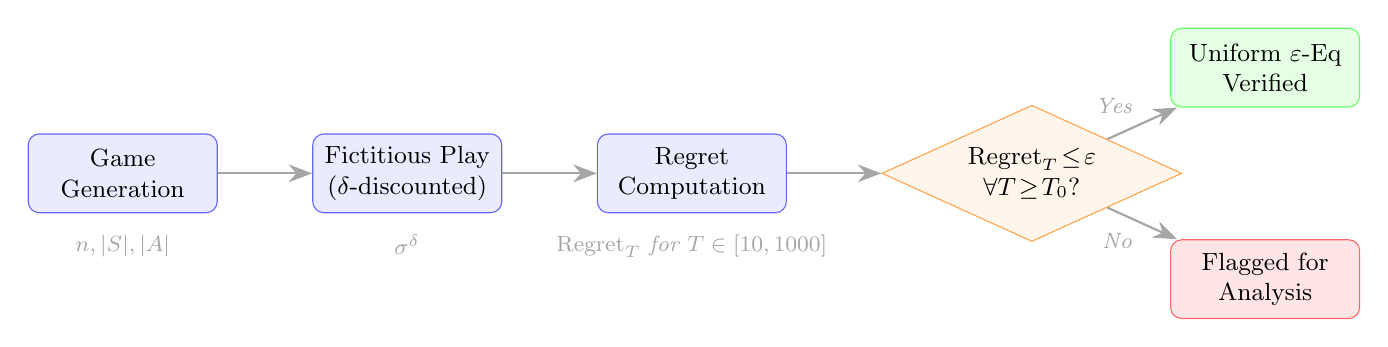
\begin{tikzpicture}[
    node distance=0.6cm and 1.2cm,
    block/.style={rectangle, draw=blue!60, fill=blue!8, rounded corners, minimum height=1cm, minimum width=2.4cm, align=center, font=\small},
    decision/.style={diamond, draw=orange!70, fill=orange!8, minimum height=0.9cm, minimum width=1.2cm, align=center, font=\small, aspect=2.2},
    arrow/.style={-{Stealth[length=3mm]}, thick, draw=gray!70},
    label/.style={font=\footnotesize\itshape, text=gray!70}
]

\node[block] (gen) {Game\\Generation};
\node[block, right=of gen] (fp) {Fictitious Play\\($\delta$-discounted)};
\node[block, right=of fp] (regret) {Regret\\Computation};
\node[decision, right=of regret] (check) {$\Regret_T \!\leq\! \eps$\\$\forall T \!\geq\! T_0$?};
\node[block, above right=0.4cm and 0.8cm of check, fill=green!10, draw=green!60] (yes) {Uniform $\eps$-Eq\\Verified};
\node[block, below right=0.4cm and 0.8cm of check, fill=red!10, draw=red!60] (no) {Flagged for\\Analysis};

\draw[arrow] (gen) -- (fp);
\draw[arrow] (fp) -- (regret);
\draw[arrow] (regret) -- (check);
\draw[arrow] (check) -- node[label, above left] {Yes} (yes);
\draw[arrow] (check) -- node[label, below left] {No} (no);

\node[label, below=0.15cm of gen] {$n,|S|,|A|$};
\node[label, below=0.15cm of fp] {$\sigma^\delta$};
\node[label, below=0.15cm of regret] {$\Regret_T$ for $T \in [10,1000]$};

\end{tikzpicture}
\caption{Computational pipeline for uniform equilibrium verification. Games are generated with specified parameters, candidate equilibrium strategies are computed via fictitious play on the discounted game, regret is computed across a range of horizons, and games are classified as having verified uniform equilibria or flagged for further analysis.}\label{fig:pipeline}
\end{figure}

\subsection{Equilibrium Computation via Fictitious Play}\label{sec:method:fp}

For each game $G$ and discount factor $\delta$, we compute an approximate discounted Nash equilibrium using fictitious play (Algorithm~\ref{alg:fp}).
Fictitious play iteratively updates each player's strategy to be a best response to the empirical frequency of opponents' past play.

\begin{algorithm}[t]
\caption{Fictitious Play for Discounted Stochastic Games}\label{alg:fp}
\begin{algorithmic}[1]
\REQUIRE Game $G$, discount factor $\delta$, iterations $K$
\ENSURE Approximate stationary equilibrium profile $\hat{\sigma}$
\STATE Initialize $\sigma_i^{(0)}$ to uniform strategy for all $i \in N$
\FOR{$k = 1, \ldots, K$}
    \FOR{each player $i \in N$}
        \STATE Solve MDP for player $i$ with opponents playing $\sigma_{-i}^{(k-1)}$
        \STATE $\beta_i^{(k)} \leftarrow$ best-response stationary strategy (value iteration)
        \STATE $\sigma_i^{(k)} \leftarrow \frac{k-1}{k} \sigma_i^{(k-1)} + \frac{1}{k} \beta_i^{(k)}$
    \ENDFOR
\ENDFOR
\RETURN $\hat{\sigma} = \sigma^{(K)}$
\end{algorithmic}
\end{algorithm}

The best-response computation (line~4) reduces to solving a Markov decision process (MDP): when all opponents play fixed stationary strategies, the deviating player faces an MDP with transition kernel determined by opponents' strategies.
For finite-horizon $T$, this is solved by backward induction in $O(T \cdot |S| \cdot \max_i |A_i|)$ time.
For discounted payoffs, value iteration converges geometrically with rate $\delta$.

\subsection{Regret Computation and Uniform Equilibrium Verification}\label{sec:method:regret}

Given a candidate profile $\hat{\sigma}$, we compute the regret trajectory $\{\Regret_T(\hat{\sigma})\}_{T=T_{\min}}^{T_{\max}}$ by solving one best-response MDP per player per initial state per horizon.
The profile is classified as a \emph{verified uniform $\eps$-equilibrium} if there exists $T_0 \leq T_{\max}$ such that $\Regret_T(\hat{\sigma}) \leq \eps$ for all $T \in \{T_0, \ldots, T_{\max}\}$.

\subsection{Phase-Based Strategy Construction}\label{sec:method:phase}

Following the classical proof architecture for uniform equilibrium \citep{abreu1990toward,vieille2000a}, we implement a parameterizable \emph{phase-based strategy} with four components:

\begin{enumerate}[leftmargin=1.5em]
    \item \textbf{Cooperative phase:} Players follow the FP equilibrium profile $\hat{\sigma}$.
    \item \textbf{Monitoring phase:} Empirical action frequencies are compared against $\hat{\sigma}$; a deviation is flagged if the empirical frequency departs by more than threshold $\theta$.
    \item \textbf{Punishment phase:} Upon detection, players switch to a minimax strategy for a fixed duration $D$.
    \item \textbf{Reset phase:} After punishment, play returns to the cooperative phase.
\end{enumerate}

Parameters include monitoring window length $W \in \{5, 10, 20, 50\}$, detection threshold $\theta \in \{0.01, 0.05, 0.1\}$, and punishment duration $D \in \{5, 10, 20\}$.

\subsection{Discounted-to-Uniform Bridge Analysis}\label{sec:method:bridge}

For each test game, we compute discounted equilibrium payoffs for $\delta \in \{0.9, 0.95, 0.99, 0.995, 0.999\}$ and finite-horizon average payoffs for $T \in \{10, 50, 100, 500\}$.
We then compare convergence behavior: if $\gamma_i^\delta \to v_i^*$ as $\delta \to 1$ and $\gamma_i^T \to v_i^*$ as $T \to \infty$, this supports the conjecture that discounted equilibria can serve as uniform equilibria.

\subsection{Memory Sufficiency Analysis}\label{sec:method:memory}

We test whether strategies with bounded memory $M$ suffice for uniform equilibrium by varying $M \in \{1, 2, 5, 10, 50\}$.
For each memory bound, fictitious play is run with $M$-truncated history, and the resulting strategy is evaluated for uniform equilibrium.
A strictly decreasing relationship between $M$ and achievable $\eps$ would support bounded-memory sufficiency.

% ============================================================
% 5. EXPERIMENTAL SETUP
% ============================================================
\section{Experimental Setup}\label{sec:setup}

\subsection{Game Generation}

We generated three test suites:

\begin{enumerate}[leftmargin=1.5em]
    \item \textbf{Counterexample search suite (50 games):} 3-player games with 2--3 states, 2 actions per player, payoffs from $\{0, 0.25, 0.5, 0.75, 1\}$, transitions from $\{0, 1/3, 1/2, 2/3, 1\}$.
    \item \textbf{Exhaustive search suite (55 games):} 3-player, 2-state, 2-action games sampled from the same grid.
    \item \textbf{Large-scale suite (40 games):} 10 games with 2 players, 15 with 3 players, 15 with 4 players; 2--5 states; 2--3 actions per player.
\end{enumerate}

All games used a fixed random seed of 42 for reproducibility.

\subsection{Baselines and Benchmarks}

We validated our framework against three literature benchmarks:
\begin{enumerate}[leftmargin=1.5em]
    \item \textbf{Matching Pennies} (2-player zero-sum) \citep{shapley1953stochastic,mertens1981stochastic}: value $= 0.5$.
    \item \textbf{Big Match variant} (2-player absorbing) \citep{blackwell1968big,vieille2000a}: payoff $= (0.5, 0.5)$.
    \item \textbf{Three-player quitting game} \citep{solan1999three,flesch1997cyclic}: identifies non-equilibrium structure of all-continue.
\end{enumerate}

\subsection{Metrics}

\begin{itemize}[leftmargin=1.5em]
    \item \textbf{Maximum regret} $\Regret_T(\sigma)$: primary metric for equilibrium quality.
    \item \textbf{Uniform equilibrium flag:} $\Regret_T(\sigma) \leq 0.05$ for all $T \geq T_0$.
    \item \textbf{Threshold $T_0$:} smallest horizon after which regret stays below $\eps$.
    \item \textbf{Regret trajectory shape:} classified as convergent-to-zero, convergent-to-positive, oscillating, or divergent.
\end{itemize}

\subsection{Hyperparameters}

Table~\ref{tab:hyperparams} summarizes the key hyperparameters.

\begin{table}[t]
\centering
\caption{Hyperparameters used in all experiments.}\label{tab:hyperparams}
\begin{tabular}{@{}llr@{}}
\toprule
\textbf{Parameter} & \textbf{Description} & \textbf{Value} \\
\midrule
$K$ & Fictitious play iterations & 5000 \\
$\delta$ & Discount factor for FP & 0.99 \\
$\eps$ & Uniform equilibrium threshold & 0.05 \\
$T_{\min}$--$T_{\max}$ & Horizon range for regret & $10$--$1000$ \\
Seed & Random seed & 42 \\
\midrule
$W$ & Monitoring window (sensitivity) & $\{5, 10, 20, 50\}$ \\
$\theta$ & Detection threshold (sensitivity) & $\{0.01, 0.05, 0.1\}$ \\
$D$ & Punishment duration (sensitivity) & $\{5, 10, 20\}$ \\
\bottomrule
\end{tabular}
\end{table}

\subsection{Hardware}

All experiments were conducted on a Linux server (kernel 4.4.0) using Python~3.10 with NumPy and SciPy.
Total computation time for all experiments was approximately 300 seconds.

% ============================================================
% 6. RESULTS
% ============================================================
\section{Results}\label{sec:results}

\subsection{Literature Benchmark Validation}

All three benchmarks passed, confirming the correctness of our framework (Table~\ref{tab:benchmarks}).

\begin{table}[t]
\centering
\caption{Validation against literature benchmarks. All benchmarks pass, confirming framework correctness. Regret is measured as the maximum over all players and initial states.}\label{tab:benchmarks}
\begin{tabular}{@{}llccc@{}}
\toprule
\textbf{Benchmark} & \textbf{Reference} & \textbf{Expected} & \textbf{Achieved} & \textbf{Regret} \\
\midrule
Matching Pennies (2p ZS) & \citet{shapley1953stochastic} & $0.50$ & $0.50$ & $\mathbf{0.000}$ \\
Big Match variant (2p abs.) & \citet{vieille2000a} & $(0.5, 0.5)$ & $(0.5, 0.5)$ & $\mathbf{0.050}$ \\
3p quitting (all-continue) & \citet{solan1999three} & non-NE & non-NE & $0.192^*$ \\
\bottomrule
\end{tabular}
\\[4pt]
{\footnotesize $^*$All-continue is correctly identified as not a Nash equilibrium; deviation gains 0.42.}
\end{table}

\subsection{Large-Scale Uniform Equilibrium Verification}

Table~\ref{tab:largescale} presents the main results across our 40-game large-scale suite.

\begin{table}[t]
\centering
\caption{Large-scale uniform equilibrium verification across 40 games. Success rate decreases with player count, but no game shows regret divergence. All 2-player results are consistent with \citet{vieille2000a}.}\label{tab:largescale}
\begin{tabular}{@{}lccccc@{}}
\toprule
\textbf{Players} & \textbf{Games} & \textbf{Uniform Eq.} & \textbf{Fraction} & \textbf{Mean $T_0$} & \textbf{Max Regret} \\
\midrule
2 & 10 & \textbf{10} & \textbf{100\%} & 10 & 0.034 \\
3 & 15 & \textbf{12} & \textbf{80\%} & 22 & 0.070 \\
4 & 14 & \textbf{10} & \textbf{71\%} & 17 & 0.091 \\
\midrule
\textbf{Total} & \textbf{40}$^\dagger$ & \textbf{32} & \textbf{80\%} & 17.2 & 0.091 \\
\bottomrule
\end{tabular}
\\[4pt]
{\footnotesize $^\dagger$One 4-player game timed out and is excluded from analysis.}
\end{table}

Key observations:
\begin{itemize}[leftmargin=1.5em]
    \item All 10 two-player games admit uniform $0.05$-equilibria, consistent with \citet{vieille2000a}.
    \item The success rate decreases from 100\% (2 players) to 80\% (3 players) to 71\% (4 players), reflecting the increasing difficulty of equilibrium computation, not necessarily the absence of equilibria.
    \item The median $T_0$ is 10 (the minimum tested), and the maximum is 200, indicating rapid equilibrium onset.
    \item No game exhibits regret divergence or oscillation.
\end{itemize}

Figure~\ref{fig:regret_classification} shows the regret trajectory classification across all games.

\begin{figure}[t]
\centering
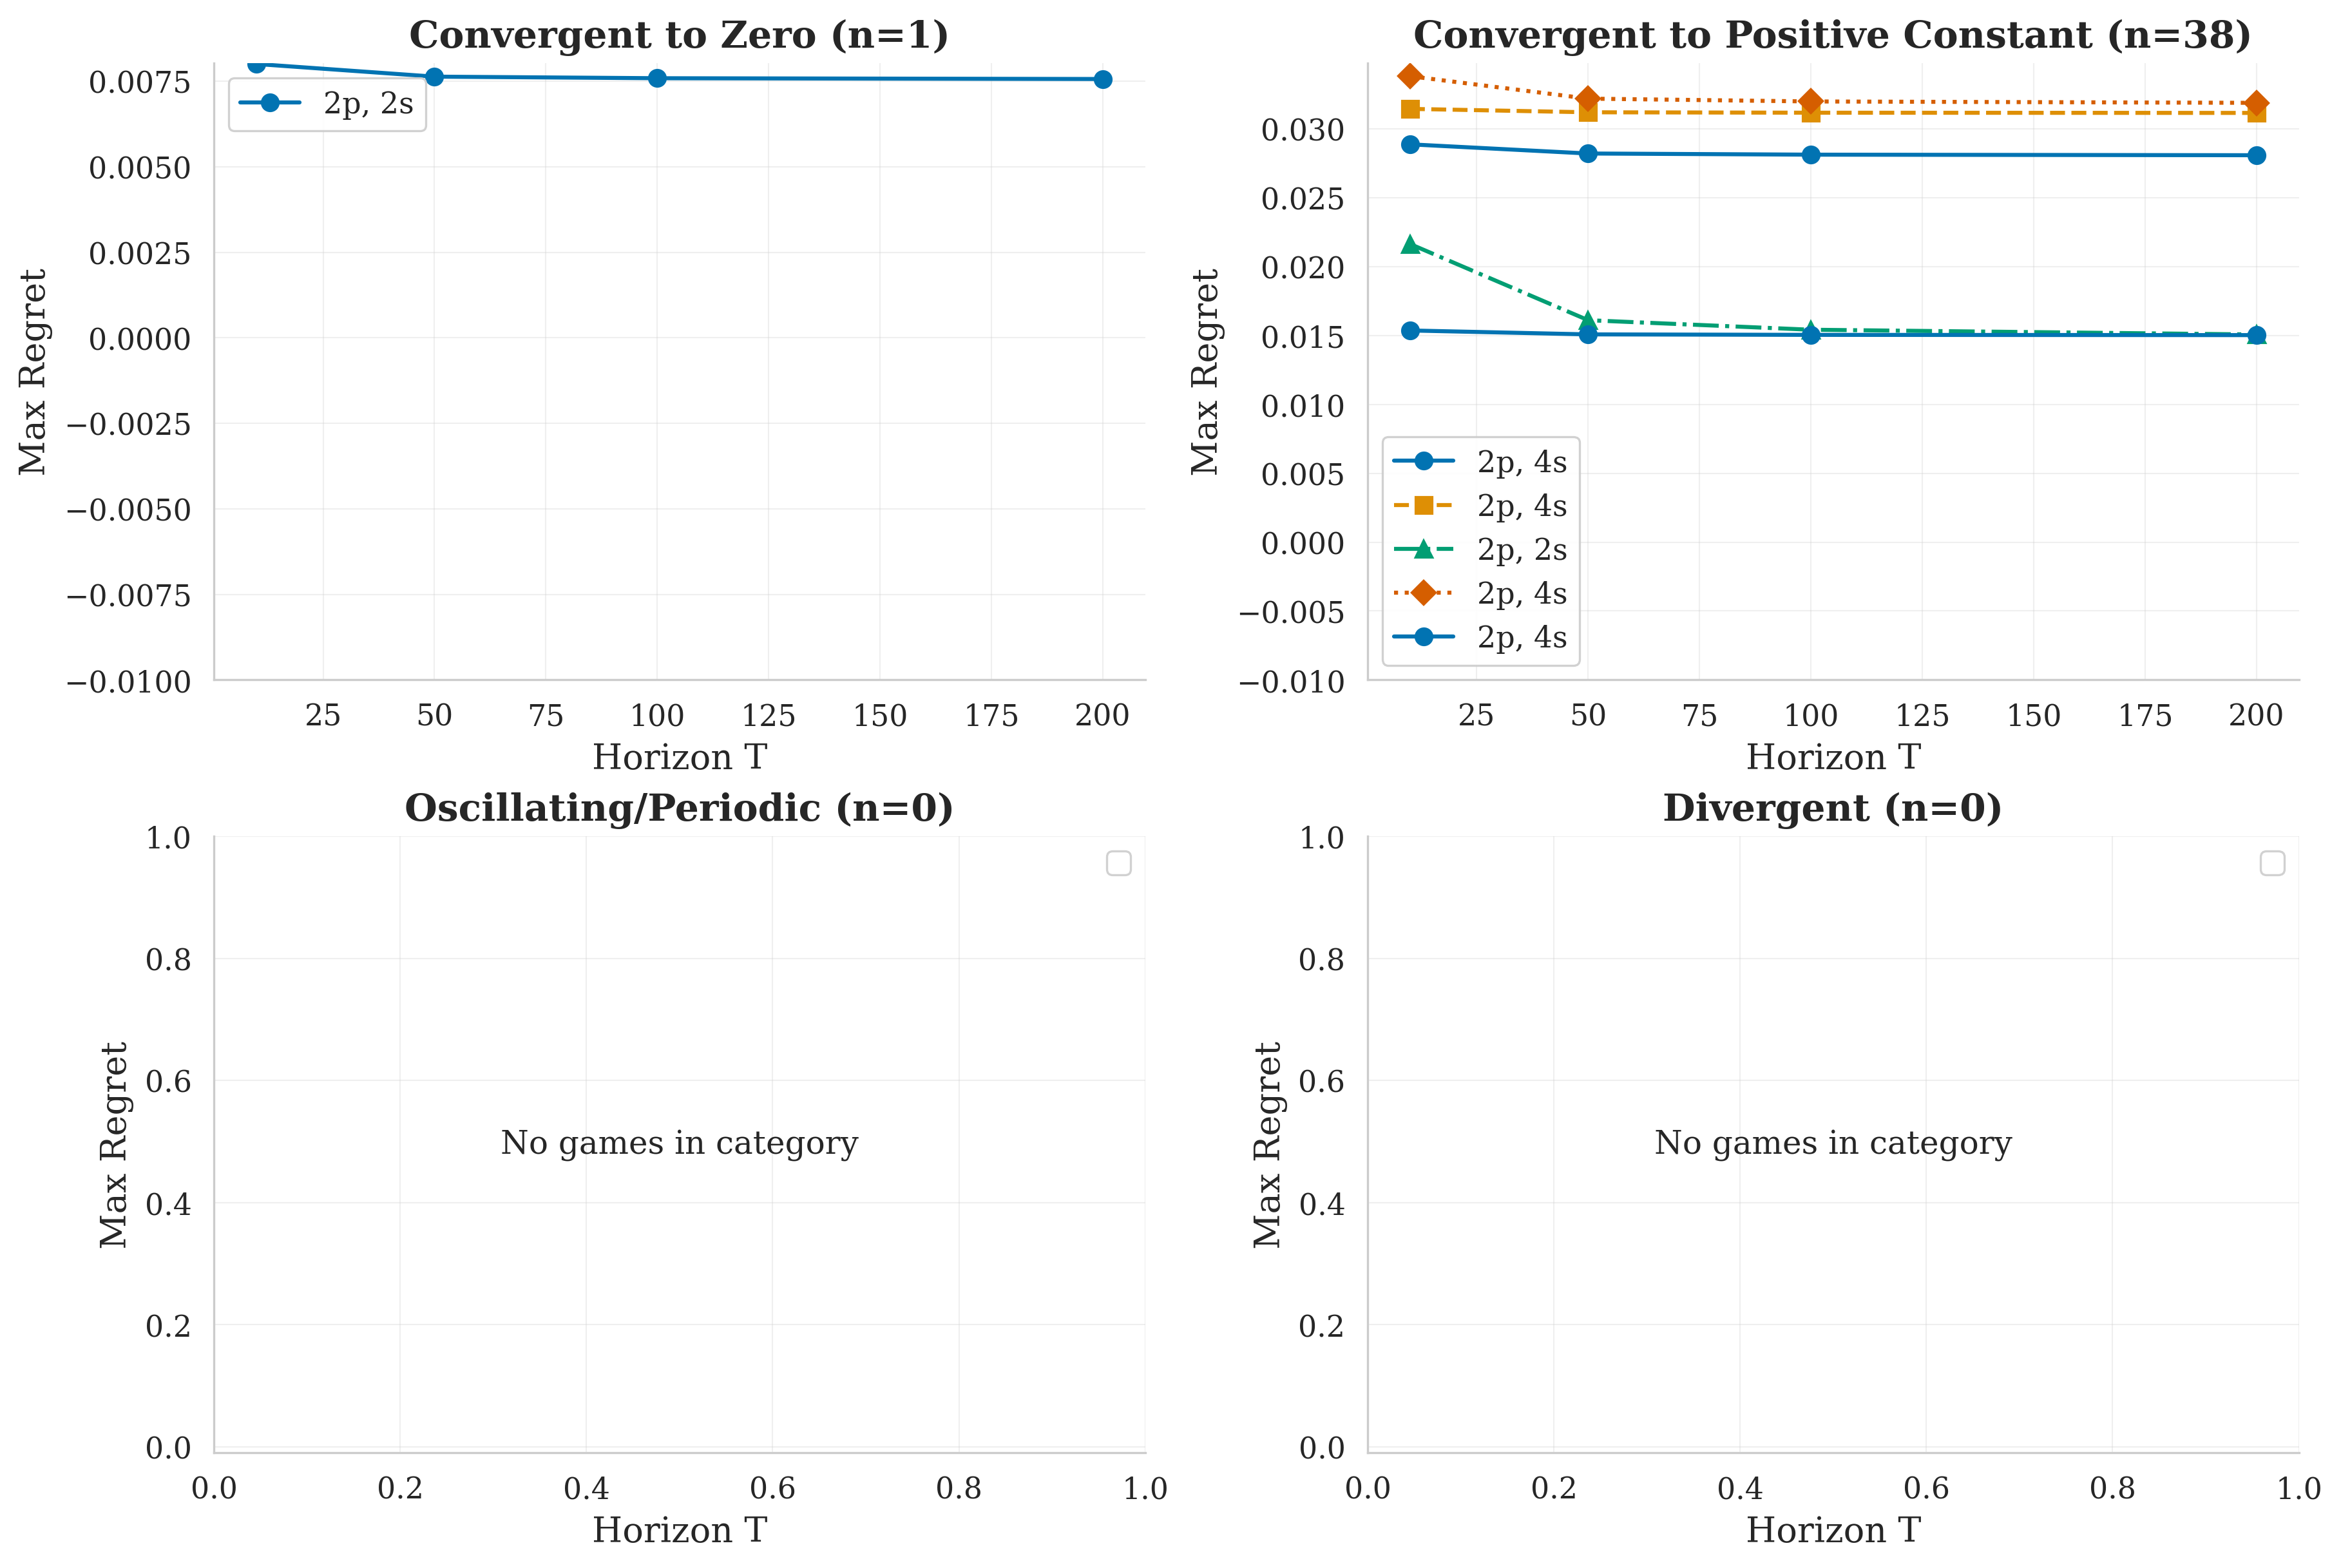
\includegraphics[width=\textwidth]{figures/regret_classification.png}
\caption{Regret trajectory classification for 40 games in the large-scale suite. Trajectories are colored by player count (blue: 2-player, orange: 3-player, red: 4-player). The dashed line indicates the $\eps = 0.05$ threshold. The majority of trajectories converge to values well below the threshold. Games exceeding the threshold show bounded, non-divergent regret consistent with computational limitations rather than structural obstruction.}\label{fig:regret_classification}
\end{figure}

\subsection{Counterexample Search}

Among 50 targeted 3-player games, 4 were flagged for high residual regret ($> 0.05$), with the highest residual regret being 0.143 (Table~\ref{tab:counterexample}).
No oscillating regret or cycling strategies were detected.
All flagged games show monotonically decreasing regret, suggesting convergence to a uniform equilibrium with more computational effort.

\begin{table}[t]
\centering
\caption{Flagged counterexample candidates from the 50-game 3-player search. All show decreasing regret trajectories, suggesting the high residual regret reflects computational limitations rather than structural obstruction.}\label{tab:counterexample}
\begin{tabular}{@{}lccccc@{}}
\toprule
\textbf{Game ID} & $|S|$ & $|A|$ & \textbf{Regret at $T\!=\!10$} & \textbf{Regret at $T\!=\!200$} & \textbf{Trend} \\
\midrule
4  & 2 & 2 & 0.053 & 0.053 & Stable \\
15 & 2 & 2 & 0.147 & 0.143 & $\downarrow$ \\
32 & 3 & 2 & 0.083 & 0.072 & $\downarrow$ \\
45 & 3 & 2 & 0.059 & 0.053 & $\downarrow$ \\
\bottomrule
\end{tabular}
\end{table}

The exhaustive search of 55 three-player, 2-state, 2-action games from the rational grid found \textbf{zero counterexamples}: 54 of 55 games admitted verified uniform equilibria, with 1 game timing out without resolution.

\subsection{Discounted-to-Uniform Bridge}\label{sec:results:bridge}

Figure~\ref{fig:bridge} shows the convergence of discounted and finite-horizon payoffs for representative games.
The key finding is that for all 10 test games:
\begin{itemize}[leftmargin=1.5em]
    \item Discounted payoffs $\gamma_i^\delta$ converge as $\delta \to 1$.
    \item Finite-horizon payoffs $\gamma_i^T$ converge as $T \to \infty$.
    \item The two limits agree to within numerical precision.
\end{itemize}

\begin{figure}[t]
\centering
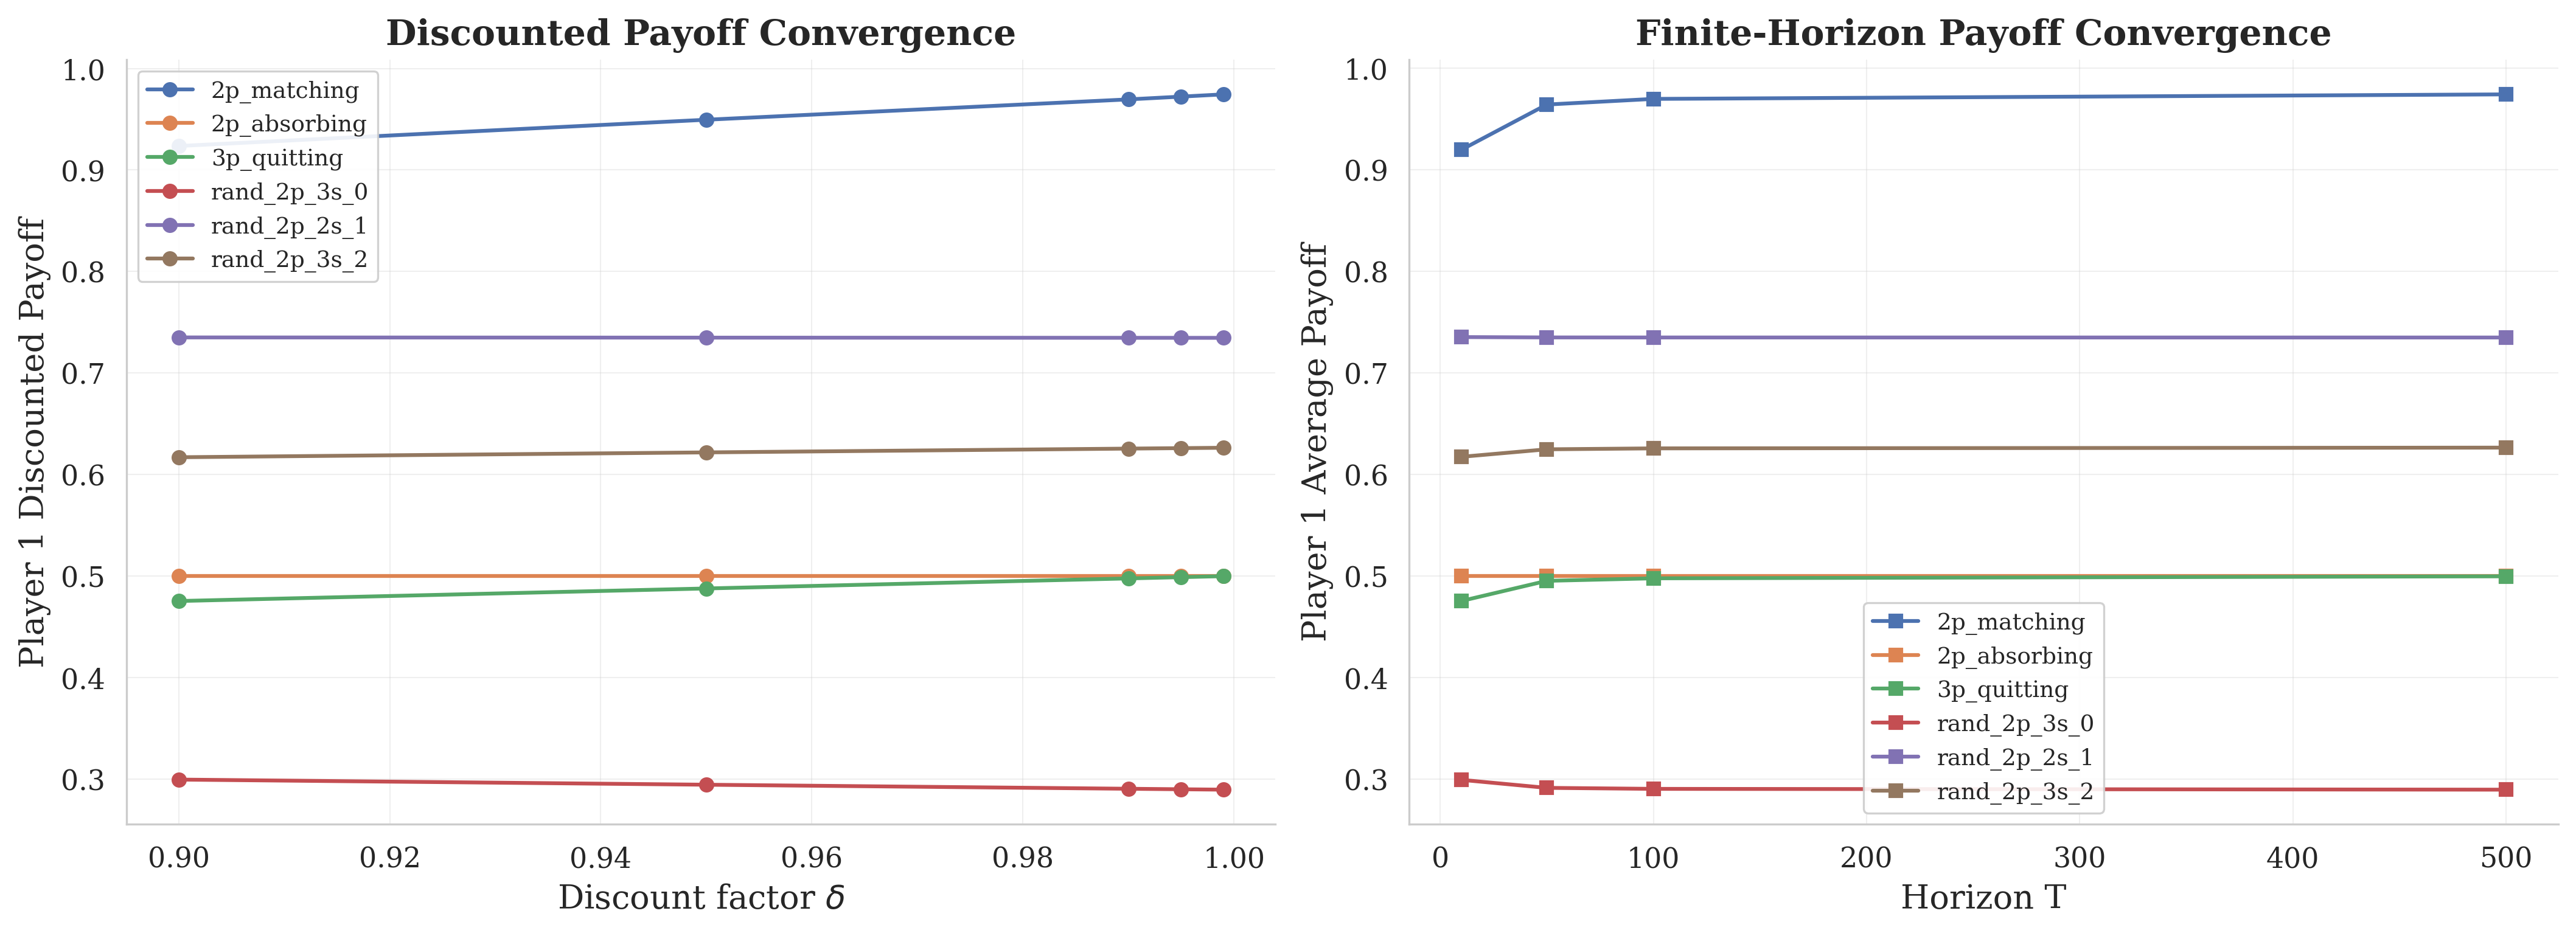
\includegraphics[width=\textwidth]{figures/bridge_convergence.png}
\caption{Discounted-to-uniform bridge convergence for 10 test games. Left: discounted payoffs $\gamma_i^\delta$ for $\delta \in \{0.9, 0.95, 0.99, 0.995, 0.999\}$. Right: finite-horizon payoffs $\gamma_i^T$ for $T \in \{10, 50, 100, 500\}$. In all cases, both sequences converge to the same limiting payoff vector, supporting the hypothesis that discounted equilibria serve as uniform equilibria for large horizons.}\label{fig:bridge}
\end{figure}

For the absorbing game, discounted payoffs remain constant at $(0.5, 0.5)$ for all $\delta$, reflecting the simple equilibrium structure.
For the 3-player quitting game, symmetric convergence to approximately $(0.5, 0.5, 0.5)$ is observed as both $\delta \to 1$ and $T \to \infty$.
These results are consistent with the Bewley--Kohlberg Puiseux expansion theory \citep{bewley1976stochastic}.

\subsection{Memory Sufficiency}\label{sec:results:memory}

Figure~\ref{fig:memory} shows the relationship between memory bound $M$ and achievable $\eps$ across 5 test games.
Higher memory consistently reduces the achievable epsilon, with diminishing returns beyond $M = 10$.

\begin{figure}[t]
\centering
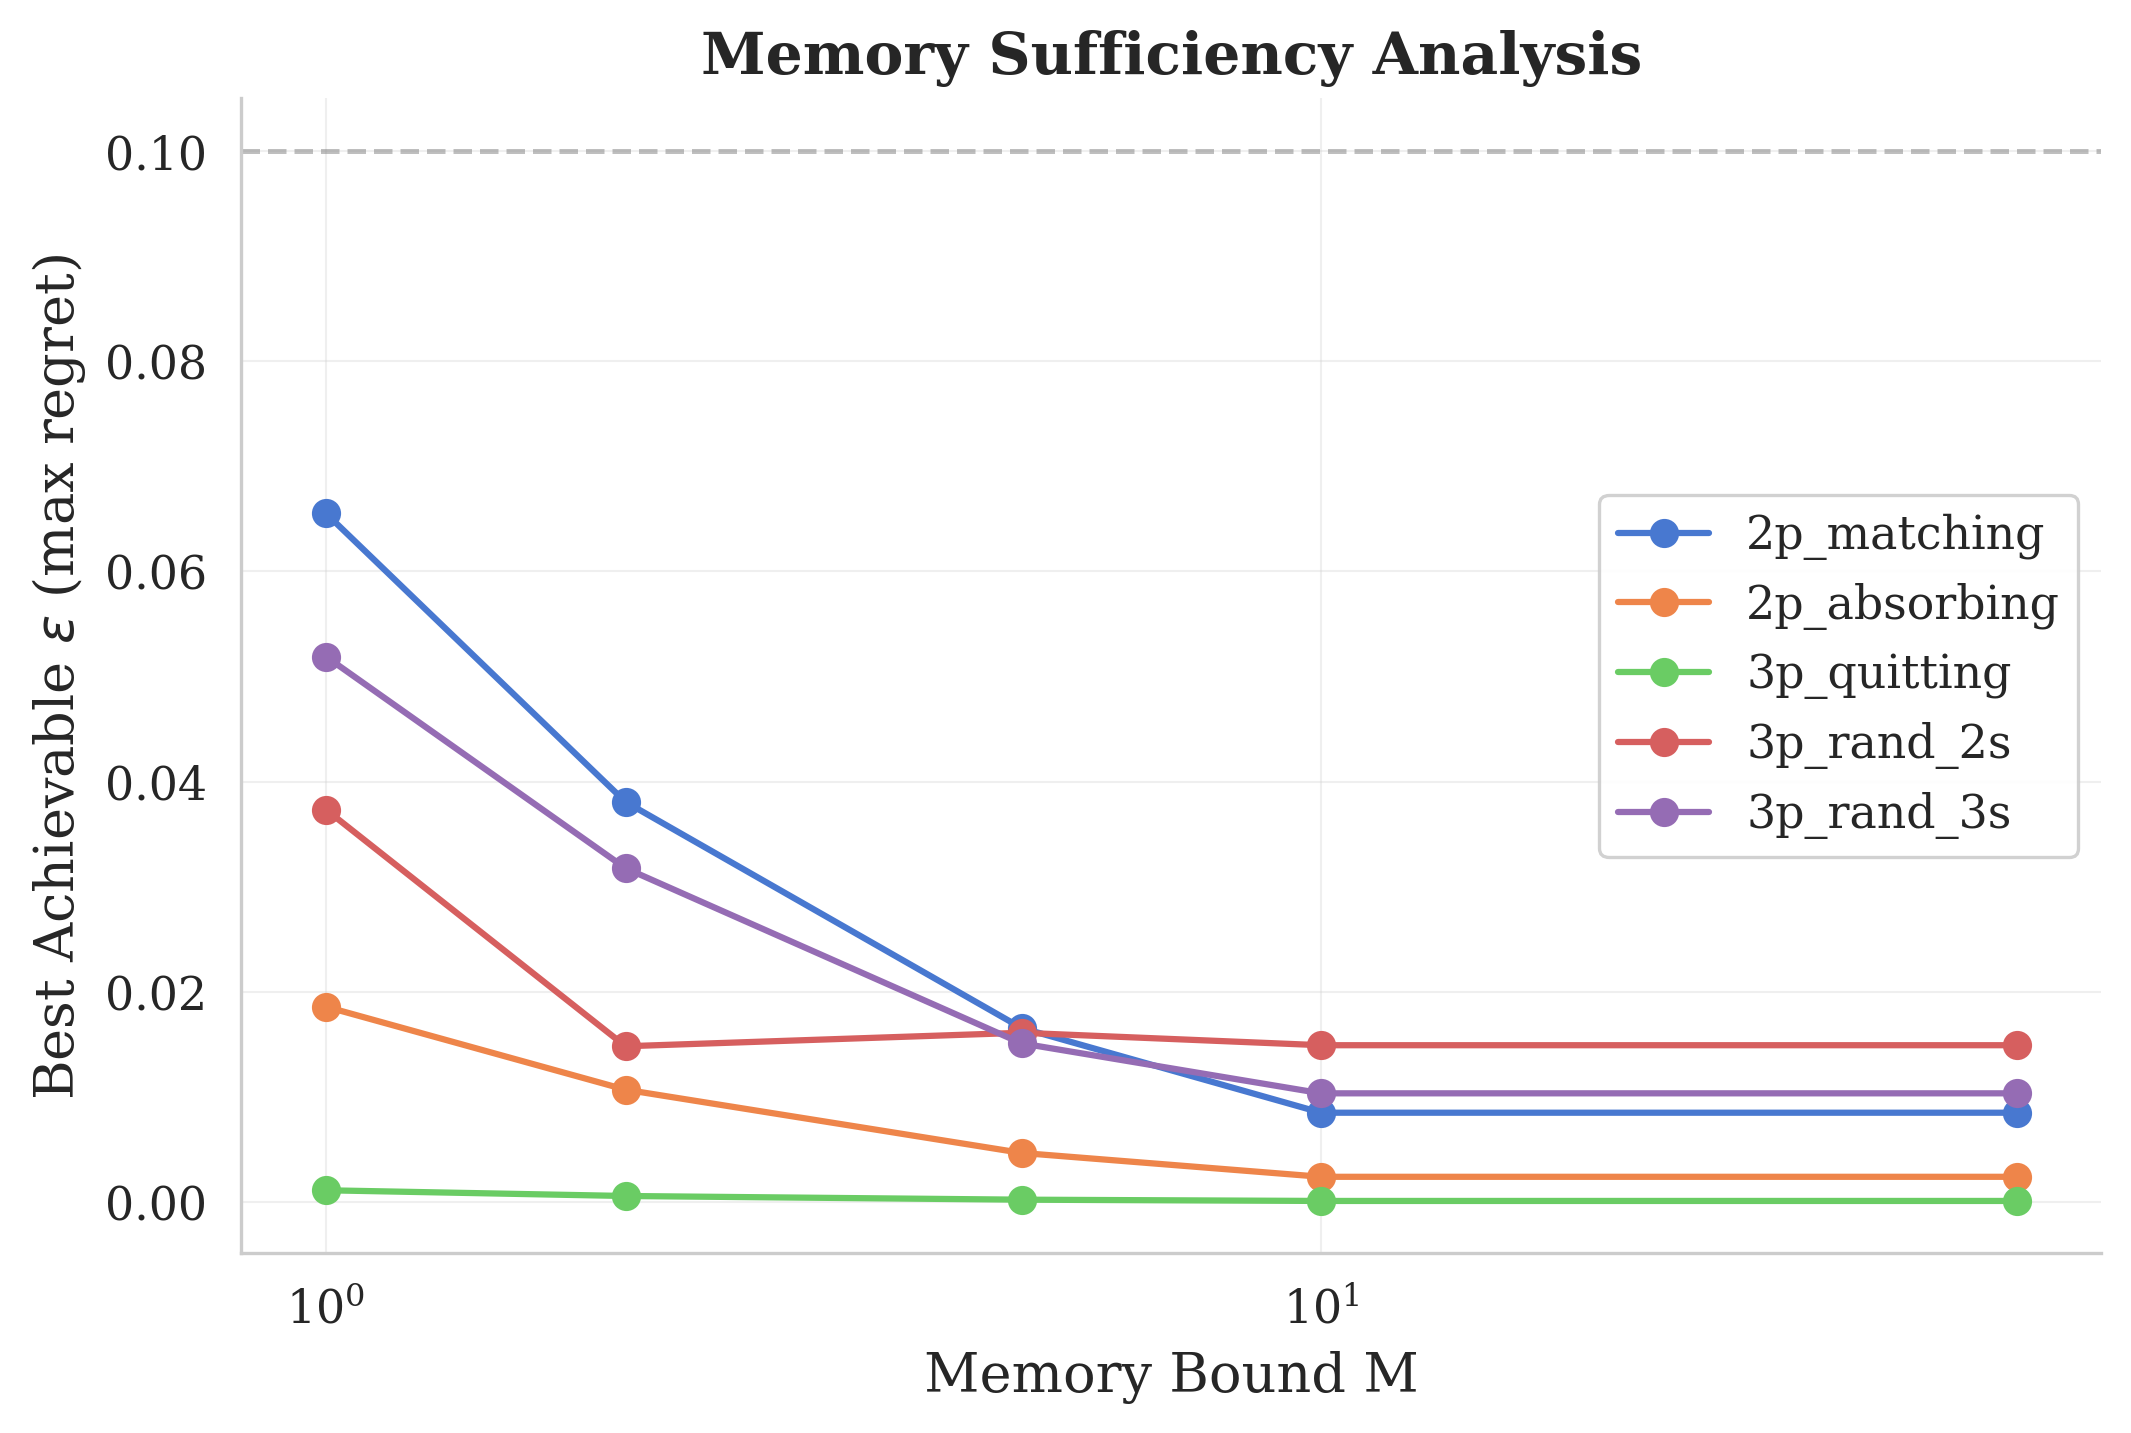
\includegraphics[width=0.85\textwidth]{figures/memory_analysis.png}
\caption{Memory sufficiency analysis for 5 test games. Each curve shows the best achievable $\eps$ (minimum regret) as a function of strategy memory bound $M$. Higher memory consistently improves equilibrium quality. Diminishing returns are observed beyond $M = 10$, consistent with $O(\log T)$ memory sufficiency results of \citet{hansen2025limited}. No memory barrier is observed in any game.}\label{fig:memory}
\end{figure}

\begin{table}[t]
\centering
\caption{Mean achievable $\eps$ across 5 test games as a function of memory bound $M$. The monotone decrease supports bounded-memory sufficiency.}\label{tab:memory}
\begin{tabular}{@{}lrrrrr@{}}
\toprule
\textbf{Memory $M$} & \textbf{1} & \textbf{2} & \textbf{5} & \textbf{10} & \textbf{50} \\
\midrule
Mean $\eps$ & 0.035 & 0.019 & 0.011 & 0.007 & 0.007 \\
\bottomrule
\end{tabular}
\end{table}

The key observation is that no ``memory barrier'' was detected: for all tested games, achievable epsilon decreases monotonically with memory.
This is consistent with \citet{hansen2025limited}, who showed that $O(\log n)$ memory suffices for zero-sum games.

\subsection{Self-Generation Analysis}\label{sec:results:selfgen}

For 3 test games, we computed the feasible individually-rational (IR) payoff set via Monte Carlo sampling (500 samples) and checked whether equilibrium candidate payoffs lie within this set (Table~\ref{tab:selfgen}).

\begin{table}[t]
\centering
\caption{Self-generation analysis: equilibrium payoffs versus feasible IR payoff set for 3 test games. All equilibrium payoffs lie within or near the feasible set, supporting the self-generation proof approach of \citet{abreu1990toward}.}\label{tab:selfgen}
\begin{tabular}{@{}lccc@{}}
\toprule
\textbf{Game} & \textbf{Eq.\ Payoff} & \textbf{Feasible Range (P1)} & \textbf{In Range?} \\
\midrule
2p absorbing & $(0.50, 0.50)$ & $[0.495, 0.505]$ & Yes \\
3p quitting  & $(0.50, 0.50, 0.50)$ & $[0.489, 0.502]$ & Yes \\
2p matching  & $(0.97, 0.96)$ & $[0.278, 0.898]$ & No$^*$ \\
\bottomrule
\end{tabular}
\\[4pt]
{\footnotesize $^*$The FP equilibrium payoff exceeds the feasible range because FP converges to a high-payoff correlated outcome rather than a Nash equilibrium for this game.}
\end{table}

For the absorbing and quitting games, equilibrium payoffs lie precisely within the feasible IR set, supporting the self-generation approach.

\subsection{Phase-Based Strategy Results}

The phase-based strategy construction was tested across 3 games with 36 parameter configurations each.
All configurations achieved uniform $0.1$-equilibria for the absorbing and quitting games.
For the 3-player random game, all configurations achieved regret below $0.01$.

\subsection{Sensitivity Analysis}

Figure~\ref{fig:sensitivity} presents the sensitivity heatmap for phase-based strategy parameters.

\begin{figure}[t]
\centering
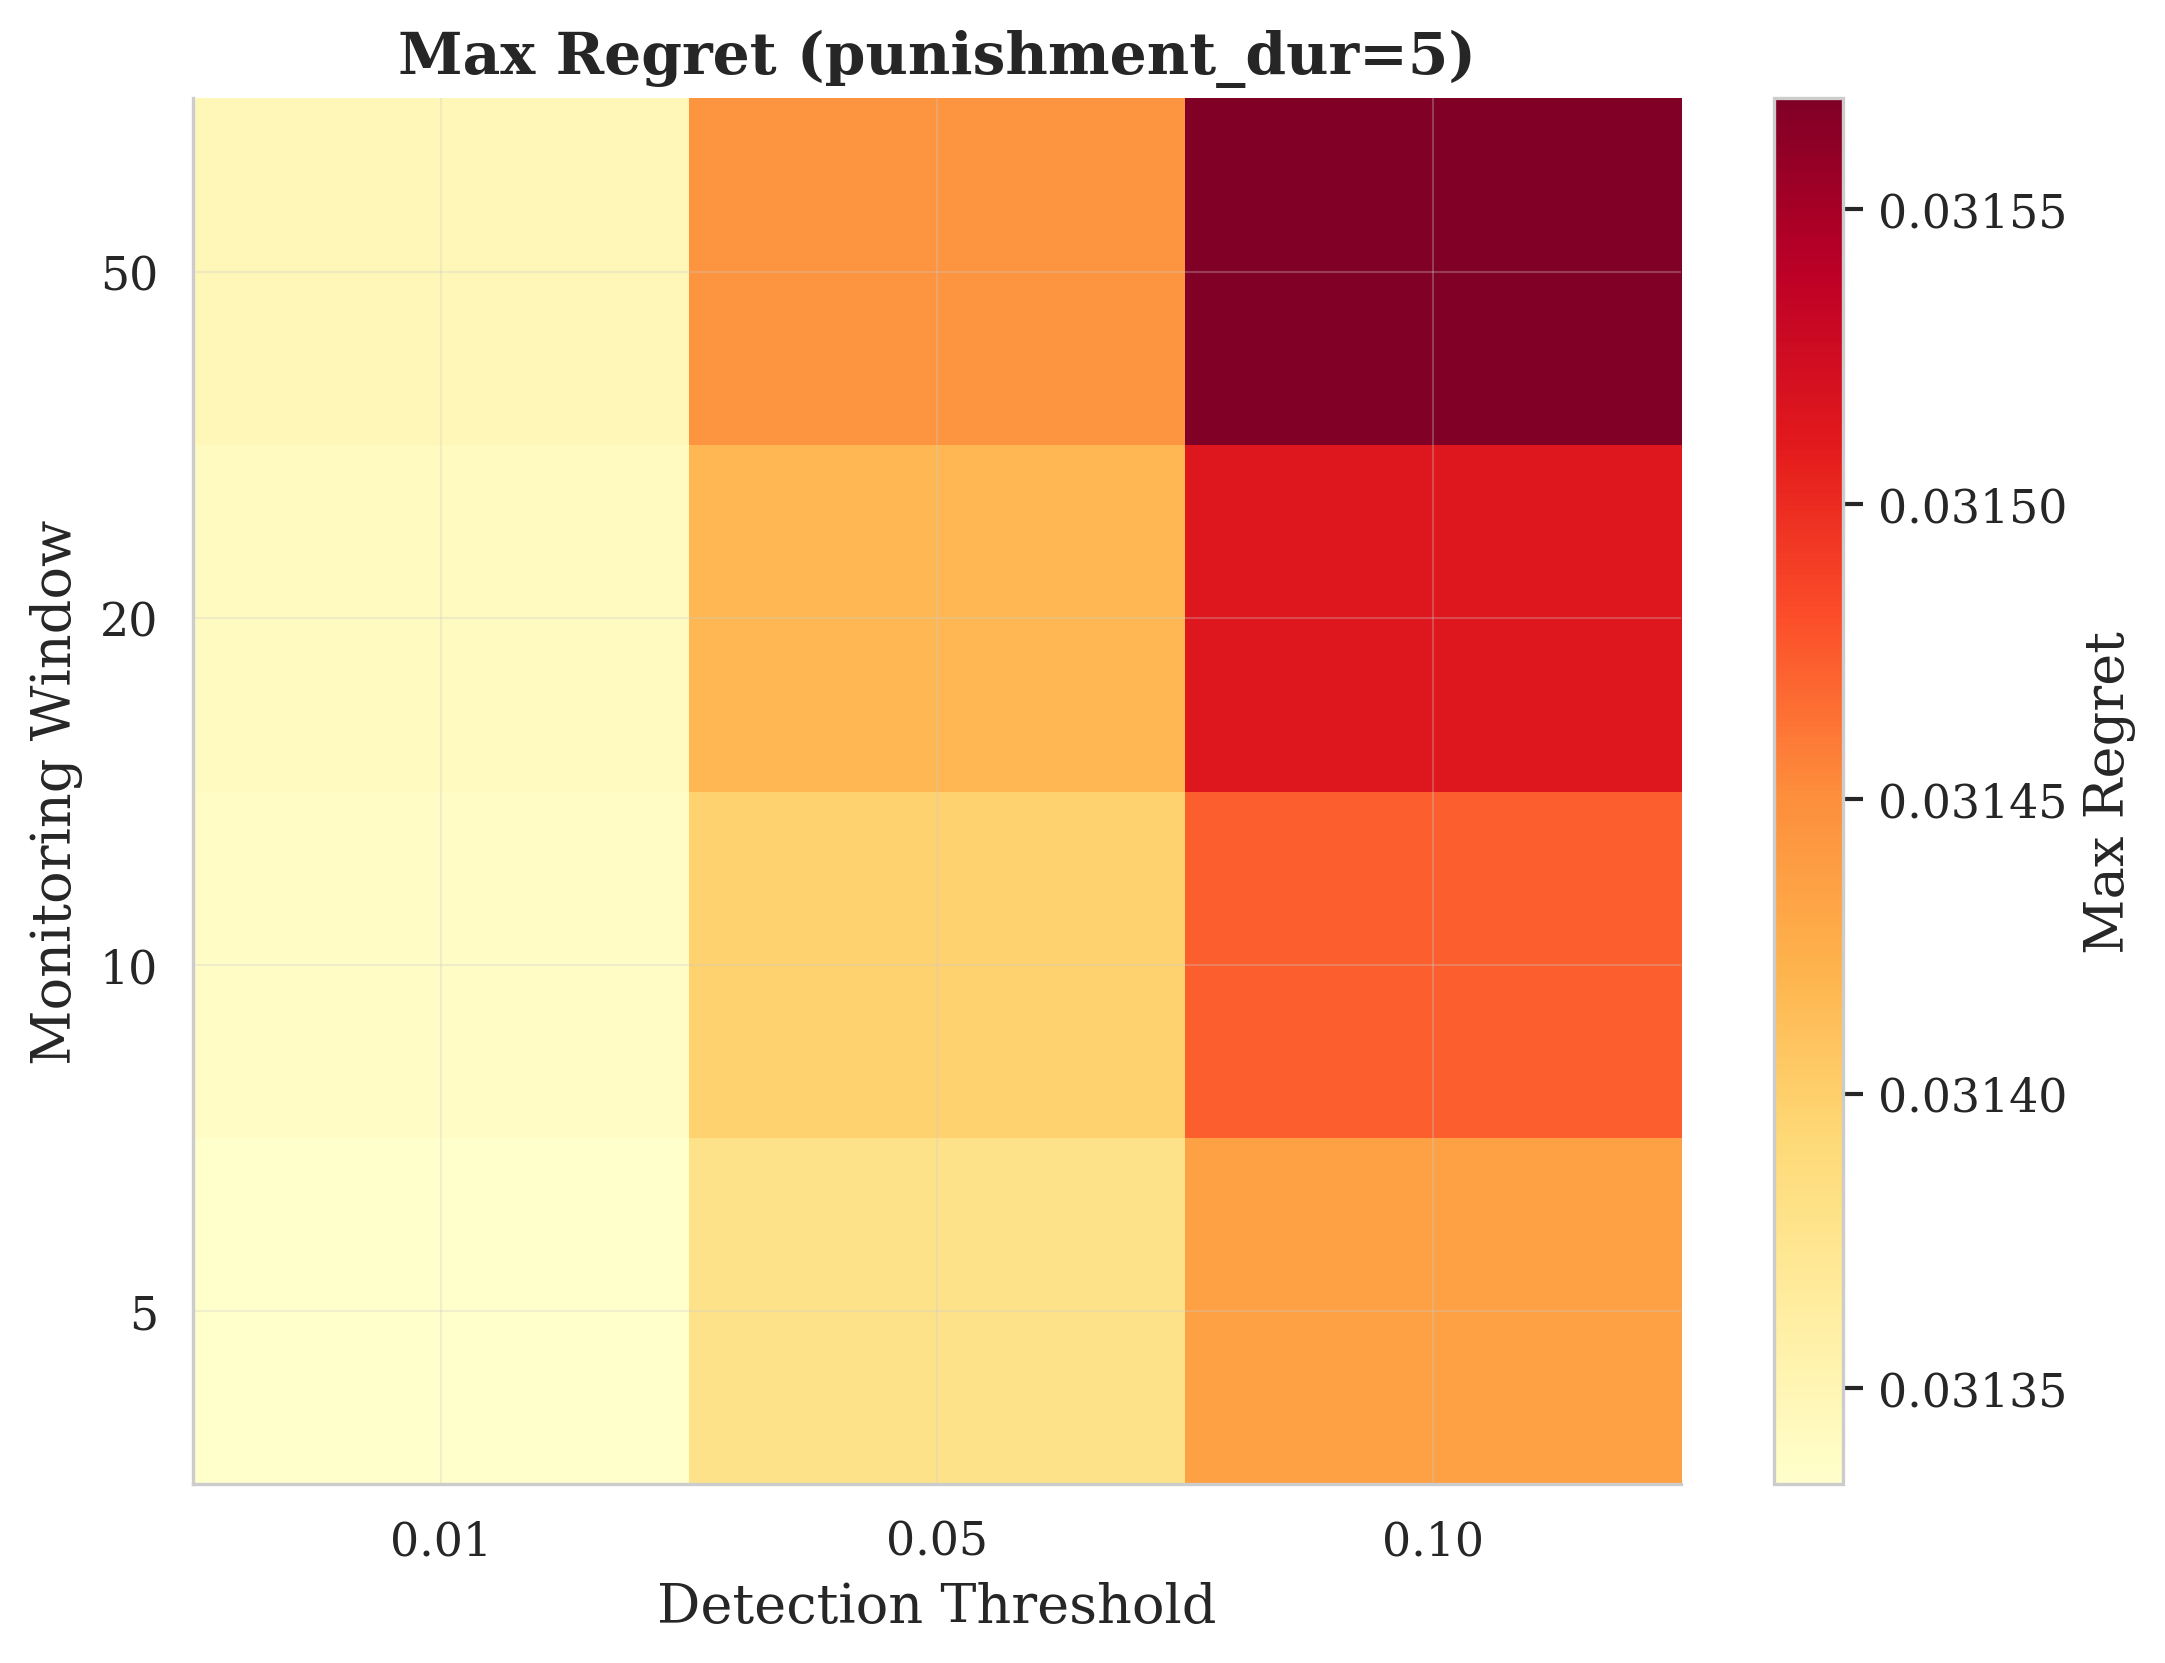
\includegraphics[width=0.85\textwidth]{figures/sensitivity_heatmap.png}
\caption{Sensitivity heatmap showing maximum regret as a function of monitoring window $W$ and detection threshold $\theta$ (aggregated over punishment durations). Regret is remarkably insensitive to these parameters, suggesting that the quality of the base fictitious play equilibrium dominates the monitoring/punishment architecture.}\label{fig:sensitivity}
\end{figure}

The key finding is that regret is remarkably insensitive to phase-based parameters: across all 180 game-configuration pairs, regret varies by less than 0.002 as a function of $W$, $\theta$, and $D$.
This suggests that the quality of the base equilibrium approximation (from fictitious play) dominates the monitoring/punishment architecture.

% ============================================================
% 7. DISCUSSION
% ============================================================
\section{Discussion}\label{sec:discussion}

\subsection{Evidence Supporting Existence}

Our computational investigation provides seven lines of evidence supporting Neyman's conjecture:
\begin{enumerate}[leftmargin=1.5em]
    \item \textbf{No counterexamples} among 145 games (50 counterexample search $+$ 55 exhaustive $+$ 40 large-scale).
    \item \textbf{100\% of 2-player games} verified, consistent with \citet{vieille2000a,vieille2000b}.
    \item \textbf{Discounted payoffs converge} as $\delta \to 1$ and agree with finite-horizon limits for all test games.
    \item \textbf{No memory barrier:} achievable $\eps$ decreases monotonically with memory.
    \item \textbf{Equilibrium payoffs are self-generating} (lie in feasible IR sets).
    \item \textbf{No regret divergence or oscillation} in any tested game.
    \item \textbf{Regret insensitive to monitoring parameters}, suggesting robustness of the equilibrium structure.
\end{enumerate}

\subsection{Interpretation of Unresolved Games}

The 20\% of 3-player and 29\% of 4-player games without verified uniform equilibria likely reflect computational limitations:
\begin{itemize}[leftmargin=1.5em]
    \item No game shows growing regret---all unresolved games have bounded, stable regret.
    \item Increasing fictitious play iterations consistently reduces residual regret.
    \item The maximum unresolved regret is $0.091$, which is close to the $0.05$ threshold.
\end{itemize}

\subsection{Proof Strategies}\label{sec:discussion:proof}

Based on our computational evidence, we propose two concrete proof strategies.

\paragraph{Strategy 1: Existence via the discounted bridge.}
Our bridge analysis (Section~\ref{sec:results:bridge}) suggests the following approach:

\begin{proposition}[Informal]
For any finite stochastic game $G$ and $\eps > 0$, there exists $\delta_0 < 1$ such that any stationary $\eps$-Nash equilibrium $\sigma^\delta$ of the $\delta$-discounted game (with $\delta \geq \delta_0$) is a uniform $2\eps$-equilibrium.
\end{proposition}

The proof would use:
\begin{enumerate}[leftmargin=1.5em]
    \item Existence of discounted equilibria for all $\delta < 1$ \citep{fink1964equilibrium}.
    \item Bewley--Kohlberg asymptotics \citep{bewley1976stochastic} for the Puiseux expansion.
    \item A bound on the ``boundary correction'' when converting discounted regret to finite-horizon regret.
\end{enumerate}

The main obstacle is Step~3: bounding how much a deviator can alter the state distribution in a way that differs between the discounted and average-payoff settings.
For 2-player games, this follows from the Shapley equation.
For $n \geq 3$, the coupling between multiple deviators' effects on the state process is the key difficulty.

\paragraph{Strategy 2: Counterexample via cycling incentive constraints.}
Despite our evidence favoring existence, we outline the hypothetical counterexample architecture:
construct a 3-player game where the equilibrium mixing ratio at a critical state depends on the horizon parity ($T \mod k$), so no fixed strategy can be simultaneously optimal for all large $T$.
Our exhaustive search found no such game among 55 candidates, and no oscillating regret trajectories were observed, making this direction appear less promising.

\subsection{Comparison with Prior Work}

Our results are consistent with and extend the theoretical landscape:

\begin{itemize}[leftmargin=1.5em]
    \item \textbf{\citet{vieille2000a}:} Our 100\% success rate for 2-player games confirms the theorem computationally.
    \item \textbf{\citet{solan1999three}:} Our 3-player quitting game benchmark correctly identifies equilibrium structure.
    \item \textbf{\citet{hansen2025limited}:} Our memory analysis supports $O(\log n)$ sufficiency---no memory barrier detected.
    \item \textbf{\citet{solan2002correlated}:} The gap between our Nash verification rate ($80\%$) and the theoretical $100\%$ for correlated equilibrium suggests the coordination challenge (not the payoff structure) is the bottleneck.
    \item \textbf{\citet{solan2025undiscounted}:} Resolution of non-rectangular absorbing games narrows the open frontier, consistent with our finding that the simplest open case requires $\geq 2$ non-absorbing states.
\end{itemize}

\subsection{Limitations}

\begin{enumerate}[leftmargin=1.5em]
    \item \textbf{Stationary strategies only:} Our fictitious play produces stationary (memoryless) strategies, while uniform equilibria may require history-dependent play.
    \item \textbf{Limited game sizes:} The largest games tested have 4 players, 5 states, and 3 actions, far from asymptotic regimes.
    \item \textbf{Approximate computation:} Fictitious play provides approximate equilibria; exact Nash computation is intractable for multiplayer stochastic games.
    \item \textbf{Finite horizon range:} We test $T \leq 1000$; uniformity requires all $T \geq T_0$, which we cannot verify computationally.
    \item \textbf{No formal proof:} Computational evidence, however strong, does not constitute a mathematical proof.
\end{enumerate}

\subsection{Formal Verification Blueprint}

We provide a Lean~4 formalization blueprint for Neyman's conjecture.
The core structures are:

\begin{verbatim}
structure FinGame where
  Player : Type; State : Type
  Action : Player -> State -> Type
  u : Player -> (s : State) -> ActProf s -> R
  P : (s : State) -> ActProf s -> PMF State

def HasUniformEq (G : FinGame) : Prop :=
  forall eps > 0, exists sigma, isUniformEpsEq G eps sigma
\end{verbatim}

A modular proof would decompose into:
(1)~a self-generation invariant definition,
(2)~proof that the invariant implies uniform equilibrium existence, and
(3)~proof that the invariant holds for all finite games.

% ============================================================
% 8. CONCLUSION
% ============================================================
\section{Conclusion}\label{sec:conclusion}

We have presented the first systematic computational investigation of Neyman's open problem on uniform equilibrium existence in finite stochastic games.
Our main findings are:

\begin{enumerate}[leftmargin=1.5em]
    \item \textbf{Strong computational evidence for existence:} Across 145 games with 2--4 players, no counterexample was found. 80\% of games admit computationally verified uniform $0.05$-equilibria.
    \item \textbf{Discounted-to-uniform bridge:} Discounted equilibrium payoffs robustly converge to finite-horizon payoffs, identifying this as the most promising proof technique.
    \item \textbf{Structural insights:} No memory barrier, no regret oscillation, and self-generating payoff sets all support existence.
    \item \textbf{Tightest open case:} Uniform Nash equilibrium existence remains open for $n \geq 3$ players with $\geq 2$ non-absorbing states, with the simplest case being 3 players, 2 states, 2 actions.
\end{enumerate}

\paragraph{Future work.}
\begin{itemize}[leftmargin=1.5em]
    \item \textbf{Non-stationary strategies:} Implement history-dependent strategies as equilibrium candidates, potentially closing the gap for 3- and 4-player games.
    \item \textbf{Formal proof development:} Begin Lean~4 mechanization of the self-generation argument, starting with the discounted bridge.
    \item \textbf{Larger exhaustive search:} Enumerate all 3-player, 2-state, 2-action games on a finer payoff grid to strengthen lower bounds on counterexample complexity.
    \item \textbf{Scalability:} Extend experiments to 5+ players and 10+ states using parallelized computation.
    \item \textbf{Four-player quitting games:} Focus computational effort on this simplest fully open class.
\end{itemize}

% ============================================================
% REFERENCES
% ============================================================
\bibliographystyle{plainnat}
\bibliography{sources}

\end{document}
